% Fair Share --- technical report
% Compile with: pdflatex docs/fair-share.tex
% (run twice if you want a resolved table of contents)
\documentclass[11pt,a4paper]{article}

\usepackage[margin=2.6cm]{geometry}
\usepackage[T1]{fontenc}
\usepackage[utf8]{inputenc}
\usepackage{lmodern}
\usepackage{microtype}
\usepackage{amsmath,amssymb}
\usepackage{booktabs}
\usepackage{tabularx}
\usepackage{enumitem}
\usepackage{graphicx}
\usepackage{xcolor}
\usepackage{hyperref}
\usepackage{url}
\usepackage{listings}
\usepackage{tikz}
\usetikzlibrary{arrows.meta,positioning,fit,calc}

\hypersetup{
  colorlinks=true,
  linkcolor=black,
  citecolor=black,
  urlcolor=blue!50!black,
  pdftitle={Fair Share: Architecture and Capabilities},
  pdfauthor={Sotirios Goulas}
}

\lstset{
  basicstyle=\ttfamily\small,
  breaklines=true,
  columns=fullflexible,
  keepspaces=true,
  showstringspaces=false,
  frame=single,
  rulecolor=\color{black!20},
  backgroundcolor=\color{black!3},
  xleftmargin=0.6em,
  xrightmargin=0.6em,
  framexleftmargin=0.4em
}

\newcommand{\fs}{\textsc{Fair Share}}
\newcommand{\code}[1]{\texttt{#1}}
\newcommand{\repo}{\texttt{fair-share}}

\title{\fs:\\Architecture and Capabilities of a Multi-Client Expense Splitter}
\author{Sotirios Goulas}
\date{September 2026\\[0.4em]\small Technical report on the \repo{} repository, version 0.1.0}

\begin{document}
\maketitle

\begin{abstract}
\fs{} is a small system for splitting trip expenses among a group of people without floating-point money.
Amounts are stored and computed as integer cents.
Equal shares use integer division with a deterministic remainder; weighted shares use the Hamilton (largest-remainder) method.
A greedy pairing of largest debtor and largest creditor produces a settlement.
The repository contains three clients that speak the same trip model: a Python command-line tool with atomic JSON persistence, a vanilla TypeScript progressive web app, and an Expo application for iOS, Android, and a web preview.
Hosted trips live behind Netlify Functions, with display JPEGs in Netlify Blobs and optional full-resolution originals in Cloudinary.
Anyone who has a trip link may edit people and expenses.
A six-digit PIN, shown once at trip creation, gates the photo gallery.
This report describes the repository layout, the money algorithms, the trust model, and the capabilities of each client.
\end{abstract}

\tableofcontents
\vspace{1.2em}
\noindent\textit{Production site:} \url{https://fair-share-trips.netlify.app}

%----------------------------------------------------------------------
\section{Purpose}
%----------------------------------------------------------------------

Splitting a shared bill looks simple until a remainder cent appears, a hotel is paid by one person and used unequally, or four people try to edit the same list from four phones.
\fs{} treats those as the product, not as afterthoughts.

The system does four things:

\begin{enumerate}[leftmargin=1.6em,itemsep=0.25em]
  \item Record who paid, how much, and who took part, using only integer cents.
  \item Compute net balances and a short list of repayments.
  \item Let a group share one trip over a URL, without accounts.
  \item Attach a PIN-gated photo gallery (``Moments'') to a hosted trip, with automatic expiry after one year.
\end{enumerate}

It does not provide user accounts, real-time collaboration locks, receipts as financial records, or in-app payments.
The mobile client may show an optional external donation link; that link is ordinary HTTPS in the system browser, not a store purchase.

%----------------------------------------------------------------------
\section{Repository layout}
%----------------------------------------------------------------------

The Git repository is a monorepo.
Money rules exist in two implementations that are intended to agree: Python under \code{src/fairshare/} for the CLI, and TypeScript under \code{packages/domain/} for the hosted stack.

\begin{table}[ht]
\centering
\caption{Top-level packages and their roles.}
\label{tab:layout}
\begin{tabular}{@{}ll@{}}
\toprule
Path & Role \\
\midrule
\code{src/fairshare/} & Python CLI: trip file, splits, settlement, \code{pull}/\code{push} \\
\code{tests/} & Pytest suite for the CLI (coverage gate 80\%) \\
\code{packages/domain/} & Shared TypeScript money, PIN, and photo constants \\
\code{web/} & Vite + TypeScript PWA (euro UI, trip links, Moments) \\
\code{netlify/functions/} & HTTP API: trips, photos, signed originals, expiry \\
\code{mobile/} & Expo SDK~57 client (same HTTP API; EAS for store builds) \\
\code{netlify.toml} & Build, functions directory, SPA rewrite for \code{/t/*} \\
\bottomrule
\end{tabular}
\end{table}

The web bundler and Vitest resolve \code{@fairshare/domain} to \code{packages/domain/src}.
Netlify Functions import the same sources by relative path and are typechecked with \code{netlify/tsconfig.json} during the production build.
The Expo app consumes the hosted JSON over HTTP; it re-exports a thin \code{mobile/src/domain} boundary and must not import server-only PIN hashing or Cloudinary signing into that barrel.

Native \code{ios/} and \code{android/} trees are not in the repository.
Store binaries are produced with EAS in the cloud.
The application identifier is \code{app.fairshare.trips}; the URL scheme is \code{fairshare}.

%----------------------------------------------------------------------
\section{Domain model}
%----------------------------------------------------------------------

A trip is a named collection of people and expenses.
Schema version is currently~$1$.
Hosted trip identifiers are 32 lowercase hexadecimal characters (16 random bytes).

An expense records a description, a payer who must already be on the trip, a positive amount in cents, a non-empty list of distinct participants, and an optional weight vector of the same length.
Person matching is case-insensitive; the first spelling seen is the canonical one.
Comma characters are forbidden in names so that CLI lists stay unambiguous.

Balances are defined in the obvious way.
If person~$p$ paid an expense of $A$ cents, $p$'s balance increases by~$A$.
Each participant $i$ is then charged share $s_i$, and $\sum_i s_i = A$ always holds because shares are computed in integer cents.

\begin{equation}
  B(p)
  \;=\;
  \sum_{\substack{e \in E \\ \mathrm{payer}(e)=p}} A_e
  \;-\;
  \sum_{\substack{e \in E \\ p \in P_e}} s_e(p).
\end{equation}

A positive balance means the group owes that person money.
A negative balance means that person owes the group.

%----------------------------------------------------------------------
\section{Algorithms}
%----------------------------------------------------------------------

\subsection{Equal split}

For an amount $A \in \mathbb{Z}_{>0}$ and $n \ge 1$ participants,

\begin{equation}
  s_i \;=\; \Bigl\lfloor \frac{A}{n} \Bigr\rfloor
  \;+\;
  \mathbf{1}\bigl[i < (A \bmod n)\bigr],
  \qquad i = 0,\ldots,n-1.
\end{equation}

The first $A \bmod n$ people receive one extra cent.
The order is the participant list as stored, so the result is deterministic and the shares sum to~$A$.

\subsection{Weighted split}

Weights $w_i$ are positive integers.
Let $W = \sum_i w_i$.
The Hamilton / largest-remainder method assigns

\begin{equation}
  q_i \;=\; \Bigl\lfloor \frac{A\, w_i}{W} \Bigr\rfloor,
  \qquad
  r_i \;=\; (A\, w_i) \bmod W,
\end{equation}

then distributes the leftover $A - \sum_i q_i$ cents one at a time to the indices with the largest $r_i$, breaking ties by earlier index.
Again $\sum_i s_i = A$, with no binary floating-point in the path.

\subsection{Settlement}

Let $B$ be the map of non-zero balances.
While both a debtor ($B < 0$) and a creditor ($B > 0$) remain, pair the most negative debtor with the most positive creditor (alphabetical name as tie-break) and transfer

\begin{equation}
  t \;=\; \min\bigl(-B(d),\, B(c)\bigr).
\end{equation}

This is a greedy min-cash-flow heuristic.
Finding a globally minimal number of transactions is NP-hard; the heuristic is used because it is simple and tends to produce a short list in practice.

\subsection{Persistence}

The CLI writes \code{fairshare.json} (or a path given by \code{--file}) by creating a temporary file in the same directory and renaming it into place.
A missing or unsupported \code{schema\_version} is a hard error.
Hosted trips are JSON documents in a Netlify Blobs store, keyed by trip id.
The public GET representation omits the PIN hash.

%----------------------------------------------------------------------
\section{Clients}
\label{sec:clients}
%----------------------------------------------------------------------

\subsection{Command-line interface}

The Python package \code{fair-share} (Python~3.11+) installs the \code{fairshare} console script.
The default data file is \code{./fairshare.json}.
Amounts accept forms such as \code{60}, \code{60.00}, \code{\$60}, and \code{\$60.50}.

\begin{table}[ht]
\centering
\caption{CLI commands.}
\label{tab:cli}
\begin{tabular}{@{}lp{8.4cm}@{}}
\toprule
Command & Effect \\
\midrule
\code{init} & Create a trip file; refuses to overwrite unless \code{--force} \\
\code{add-person} & Append one or more people \\
\code{add} & Record an equal or weighted expense \\
\code{edit-expense} & Replace an expense by full id or unique prefix \\
\code{remove-expense} & Delete an expense by id or unique prefix \\
\code{list} & Print expenses \\
\code{balances} & Print net balances \\
\code{settle} & Print who pays whom \\
\code{pull} & Download a hosted trip (money only) into the local file \\
\code{push} & Upload the local file as a \emph{new} hosted trip \\
\bottomrule
\end{tabular}
\end{table}

\code{pull} and \code{push} talk to the same HTTP API as the website.
The host is \code{--host} or the environment variable \code{FAIRSHARE\_API}.
The JSON file never contains photos or a PIN hash.
\code{push} always creates a new hosted trip and prints a fresh link and PIN.

\subsection{Web application}

\code{web/} is a cream-and-brown progressive web app built with Vite.
Currency display is euro.
Creating a trip yields a shareable path \code{/t/<id>}.
The home page lists trips seen on that device, creates a new trip, and can \textbf{Open JSON} to import people and expenses into a new hosted trip (new id, new PIN).

On a trip page a person can add and remove people, add, edit, and delete expenses, inspect balances and settlement, copy the trip link and the PIN, and \textbf{Download JSON} (money only).
Moments is the photo gallery: unlock with the PIN, upload a compressed JPEG, delete a photo, and---when Cloudinary is configured---open a short-lived original URL.

Local development is \code{npx netlify dev} on port~8888, which fronts the Vite dev server and the Functions.

\subsection{Mobile application}

\code{mobile/} is Expo Router (SDK~57).
It opens a trip by id or pasted link, then offers the same money operations and Moments against the production (or configured) API origin, defaulting to \url{https://fair-share-trips.netlify.app}.

Photo session tokens are stored with Expo SecureStore (an injectable store is used in tests).
The root layout waits until that store is ready before rendering the stack, so a cold start does not race a missing token.
Relative photo URLs from the API are prefixed with the API base.
The Support button appears only when \code{EXPO\_PUBLIC\_DONATE\_URL} (or \code{expo.extra.donateUrl}) is a non-empty HTTPS URL.

%----------------------------------------------------------------------
\section{Hosted service}
%----------------------------------------------------------------------

Production is a Netlify site.
The build installs root and \code{web} dependencies, typechecks Functions, and publishes \code{web/dist}.
SPA routes \code{/t/*} rewrite to \code{index.html}.
Response headers include \code{X-Frame-Options: DENY}, \code{X-Content-Type-Options: nosniff}, and a strict-origin referrer policy.
Functions send CORS headers including \code{Authorization}, so the Expo web preview can call the API; native \code{fetch} does not use CORS.

\begin{table}[ht]
\centering
\caption{HTTP surface (Netlify Functions).}
\label{tab:api}
\begin{tabular}{@{}llp{6.6cm}@{}}
\toprule
Method & Path & Purpose \\
\midrule
\code{POST} & \code{/api/trips} & Create trip; returns id, public trip, PIN, photo token \\
\code{GET}  & \code{/api/trips/:id} & Public trip (no PIN hash); \code{photos\_locked} if a hash exists \\
\code{PUT}  & \code{/api/trips/:id} & Replace people and expenses (link is authority) \\
\code{POST} & \code{/api/trips/:id/session} & Exchange PIN for a photo session token \\
\code{POST} & \code{/api/trips/:id/pin} & Set PIN once on a grandfathered trip \\
\code{GET}  & \code{/api/trips/:id/photos} & List gallery (PIN session if locked) \\
\code{POST} & \code{/api/trips/:id/photos} & Upload compressed display JPEG \\
\code{POST} & \code{/api/trips/:id/photos/sign} & Signed Cloudinary upload parameters \\
\code{DELETE} & \code{/api/trips/:id/photos/:photoId} & Remove display blob and original, if any \\
\code{GET}  & \code{/uploads/photos/:tripId/:photoId} & Serve display JPEG (signed query when locked) \\
\bottomrule
\end{tabular}
\end{table}

A scheduled function expires photos older than 365 days and destroys any linked Cloudinary original.

JSON bodies are capped at 200\,KiB.
Display uploads are capped at 4\,MiB and 100 photos per trip; the client compresses to a longest edge of 1600 pixels.
Originals, when enabled, allow JPEG, PNG, and HEIC/HEIF up to 15\,MiB, stored as Cloudinary \emph{authenticated} assets.
Signed original URLs last one hour.
Display URLs for locked trips are HMAC-signed and last one hour.
Photo session tokens last 30 days.

Creating a trip requires \code{PHOTO\_PIN\_PEPPER} in the environment.
Cloudinary keys are optional: without them, gallery upload still stores the compressed JPEG and \code{originalUrl} remains empty.

\begin{figure}[ht]
\centering
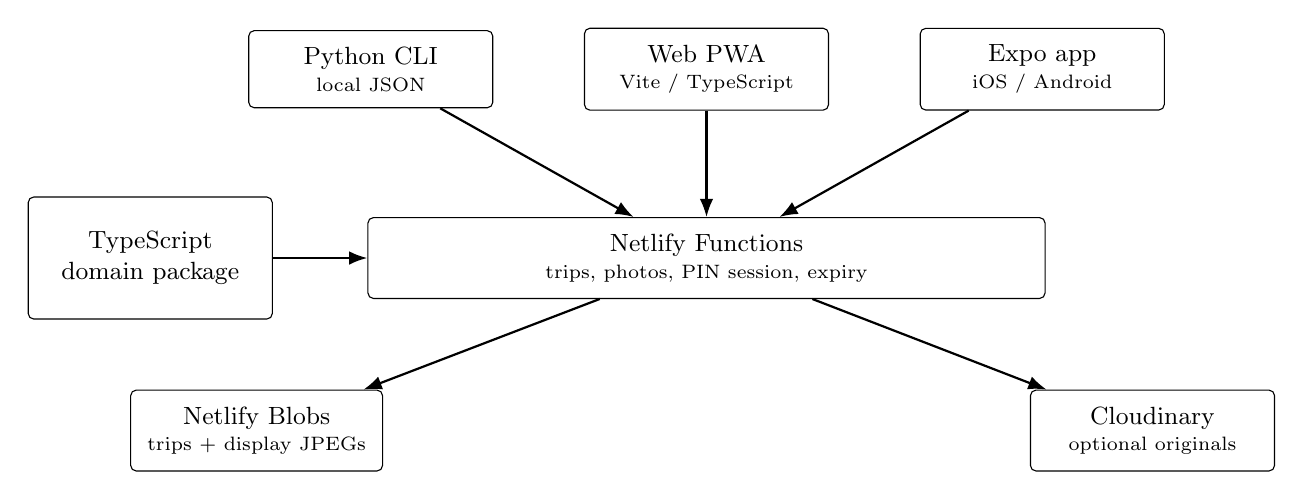
\begin{tikzpicture}[
  font=\small,
  box/.style={draw, rounded corners=2pt, align=center, inner sep=6pt, minimum width=3.1cm},
  arr/.style={-{Latex}, thick}
]
  \node[box] (cli) {Python CLI\\[-0.15em]{\scriptsize local JSON}};
  \node[box, right=1.15cm of cli] (web) {Web PWA\\[-0.15em]{\scriptsize Vite / TypeScript}};
  \node[box, right=1.15cm of web] (mob) {Expo app\\[-0.15em]{\scriptsize iOS / Android}};

  \node[box, below=1.35cm of web, minimum width=8.6cm] (api) {Netlify Functions\\[-0.15em]{\scriptsize trips, photos, PIN session, expiry}};

  \node[box, below left=1.15cm and -0.2cm of api] (blobs) {Netlify Blobs\\[-0.15em]{\scriptsize trips + display JPEGs}};
  \node[box, below right=1.15cm and -0.2cm of api] (cld) {Cloudinary\\[-0.15em]{\scriptsize optional originals}};

  \node[box, left=1.2cm of api, minimum height=1.55cm] (dom) {TypeScript\\domain package};

  \draw[arr] (cli) -- (api);
  \draw[arr] (web) -- (api);
  \draw[arr] (mob) -- (api);
  \draw[arr] (api) -- (blobs);
  \draw[arr] (api) -- (cld);
  \draw[arr] (dom) -- (api);
\end{tikzpicture}
\caption{Hosted data path.
The CLI also reads and writes a local trip file; \code{pull}/\code{push} are the only CLI calls into the Functions.
The TypeScript domain package is the money and PIN implementation for Functions, web, and (via HTTP) mobile.}
\label{fig:arch}
\end{figure}

%----------------------------------------------------------------------
\section{Trust and security model}
%----------------------------------------------------------------------

There are no accounts.
Possession of the 32-character trip id is permission to read and rewrite people and expenses.
The id is unguessable in ordinary use; it is not a secret against someone who already has the link.
That is intentional: a shared trip is meant to be edited by everyone on the holiday.

Photos are the exception.
A six-digit PIN is generated at trip creation, hashed with SHA-256 over \code{pepper:tripId:pin}, and stored beside the trip.
The pepper is a server secret (\code{PHOTO\_PIN\_PEPPER}).
Unlocking Moments issues an HMAC session token bound to the trip.
PIN guesses are rate-limited per IP.
Trips created before PIN hashing existed can set a PIN once (\code{POST .../pin}); until then, the gallery behaves as unlocked.

The PIN is shown to whoever creates the trip (and can be copied from the trip page).
It is not in the downloadable JSON.
Losing it means losing gallery administration on a locked trip; expenses remain editable via the link.

Secrets do not belong in the repository.
Local Functions read \code{.env}; production reads the Netlify UI.
\code{.env} is gitignored; \code{.env.example} lists names only.

%----------------------------------------------------------------------
\section{Capabilities, by concern}
%----------------------------------------------------------------------

\begin{table}[ht]
\centering
\caption{What each surface can do.}
\label{tab:caps}
\begin{tabular}{@{}lccc@{}}
\toprule
Capability & CLI & Web & Mobile \\
\midrule
Create a local trip file & yes & --- & --- \\
Create a hosted trip & via \code{push} & yes & yes \\
Add / edit / remove expenses & yes & yes & yes \\
Equal and weighted splits & yes & yes & yes \\
Balances and settlement & yes & yes & yes \\
Share by URL & after \code{push} & yes & yes \\
Import / export money JSON & \code{pull}/\code{push} & yes & --- \\
Photo gallery (Moments) & --- & yes & yes \\
Set PIN on a legacy trip & --- & yes & yes \\
Optional Cloudinary original & --- & yes & yes \\
Offline-first local file & yes & --- & --- \\
\bottomrule
\end{tabular}
\end{table}

``Import / export money JSON'' on the web is Download JSON on the trip page and Open JSON on the home page.
The CLI equivalents are \code{pull} (into the current file) and \code{push} (always a new hosted trip).
Photos never travel in that file.

%----------------------------------------------------------------------
\section{Development, tests, and deployment}
%----------------------------------------------------------------------

Continuous integration runs on GitHub Actions for \code{main} and pull requests:

\begin{itemize}[leftmargin=1.6em,itemsep=0.2em]
  \item Python 3.11--3.13: Ruff, then Pytest with an 80\% coverage floor on \code{fairshare}.
  \item Web: Vitest, then a production Vite build.
  \item Mobile: Vitest and \code{tsc --noEmit}.
\end{itemize}

The site deploys from the linked Netlify project.
A production CLI deploy builds Functions and \code{web/dist} and publishes to \url{https://fair-share-trips.netlify.app}.

Store submission is outside the Netlify path.
It needs an Expo account, \code{eas-cli} login and init, and App Store Connect / Play Console accounts.
The first review is expected to keep the donation URL empty if the recipient is the developer rather than a registered nonprofit.

%----------------------------------------------------------------------
\section{Limits and non-goals}
%----------------------------------------------------------------------

\begin{itemize}[leftmargin=1.6em,itemsep=0.35em]
  \item Concurrent PUT of a trip is last-write-wins.
        There is no operational transform and no per-field merge.
  \item Settlement is heuristic, not a proven minimum transfer set.
  \item Setting a PIN on a grandfathered trip re-reads before write to shrink the race; it is not a compare-and-swap.
  \item Display photos are compressed; the original is optional infrastructure, not a guarantee.
  \item The CLI money engine is Python; the hosted engine is TypeScript.
        They are kept in agreement by tests and review, not by a single compiled artefact.
  \item The product is not a bank, not a receipt archive, and not an identity provider.
\end{itemize}

%----------------------------------------------------------------------
\section{Licence}
%----------------------------------------------------------------------

The software is released under the MIT License (copyright 2026).
See \code{LICENSE} in the repository root.

%----------------------------------------------------------------------
\section{Summary}
%----------------------------------------------------------------------

\fs{} is a trip splitter whose money path never leaves the integers, whose hosted collaboration is a secret URL rather than an account system, and whose photos sit behind a PIN and a retention clock.
The repository packages that idea as a CLI for files, a PWA and an Expo app for shared links, and a small Netlify API in front of Blobs and optional Cloudinary.
The capabilities in Section~\ref{sec:clients} and Table~\ref{tab:caps} are the product; everything else is scaffolding to keep a cent from disappearing.

\end{document}
